% !Mode:: "TeX:UTF-8"

\titlepage

% \begin{frame}{说在前面}
% 	\linespread{1.5}
% 	  \begin{itemize}[<+-|alert@+>]
% 	    \item 过往的作业只画$\color{red}\times$和划线,不画$\color{red}\surd$,
% 	    最后写{\bb “查”};
% 	    \item 就近订正,方便查阅,用不同颜色的笔;
% 	    \item 不要忘记贴照片,作业本封面注明学员队和班号!
% 	    \item 作业本不要分栏写!
% 	    \item 不要当“复印机”!
% 	    \item 作业晚交、进度过慢或缺题过多最高得$\b B$,
% 	    不交默认为$\b C$!
% % 	    \item {\b 今后每周一交作业,按照单双周对应学号尾数为单双号的同学分别上交,
% % 	    平均每人两周交一次作业。} 
% 	  \end{itemize}
% \end{frame}

\begin{frame}{出现的问题}
	\linespread{1.5}
	  \begin{itemize}[<+-|alert@+>]
	    \item 求导题
	    \begin{itemize}
	      \item \b\it $y^n$和$y^{(n)}$混淆
	      \item \b\it 分段定义的函数分段点处的导数值没有用定义计算
	    \end{itemize}
	    \item 应用题
	    \begin{itemize}
	      \item \b\it $x'(t)=5$,故$x(t)=5t$ \ba{$\times$}
	      \item \b\it 无图无文字,让人如何看得懂?!
	    \end{itemize}
	  \end{itemize}
\end{frame}

\section{2.3 高阶导数}

\begin{frame}
	\linespread{1.5}
	\ba{2.已知$f(x)$二阶可导,设$y=\df{f(x)}{x}$,求$\df{\d^2y}{\d x^2}$。}
	\pause
	
% 	\bigskip
	
	解:\it
	\begin{align*}
		y'&=\df{f'(x)x-f(x)}{x^2},\\
		y''&=\df{f''(x)x^3-2x[f'(x)x-f(x)]}{x^4}\\
		&=\df{f''(x)x^2-2f'(x)x+f(x)}{x^3}.
	\end{align*}
	\hfill$\Box$
\end{frame}

\begin{frame}
	\linespread{1.5}
	\ba{3.已知$f(x)=\left\{\begin{array}{ll}
	  	\ln(1+2x),& x>0, \\ x^2+2x, & x\leq 0,
	  \end{array}\right.$
	求$f''(x)$。}\pause
	
	\bigskip
	
	\small 解:\it 
	$x>0$时,$f'(x)=\df2{1+2x}$;$x<0$时,$f'(x)=2x+2$,
	\pause 又
	$$f'_-(0)=\lim\limits_{\Delta x\to0^-}\df{\Delta x^2+2\Delta x-0}{\Delta x}=2.$$
	$$f'_+(0)=\lim\limits_{\Delta x\to0^+}\df{\ln(1+2\Delta x)-0}{\Delta x}=2.$$
	故$f'(0)=2$。
\end{frame}

\begin{frame}
	\linespread{1.5}
% 	\ba{3.已知$f(x)=\left\{\begin{array}{ll}
% 	  	\ln(1+2x),& x>0, \\ x^2+2x, & x\leq 0,
% 	  \end{array}\right.$
% 	求$f''(x)$。}\pause
	
% 	\bigskip
	
	\small \it 
	进而,当$x>0$时,$f''(x)=-\df4{(1+2x)^2}$;当$x<0$时,$f''(x)=2$,
	\pause 又
	$$f''_+(0)=\lim\limits_{\Delta x\to0^+}
	\df{\frac2{1+2\Delta x}-2}{\Delta x}
	=\lim\limits_{\Delta x\to0^+}
	\df{-4}{1+2\Delta x}=-4,$$
	$$f''_+(0)=\lim\limits_{\Delta x\to0^+}
	\df{2\Delta x+2-2}{\Delta x}=2,
	$$
	故$f''(0)$不存在。综上
	$$f''(x)=\left\{\begin{array}{ll}
		-\df4{(1+2x)^2}, & x>0;\\
		2, & x<0.
	\end{array}\right.$$
	\hfill$\Box$
\end{frame}

\begin{frame}
	\linespread{1.5}
	\ba{4.求下列函数的$n$阶导函数:(1)$y=\sin^2x$}\pause
	
	\bigskip
	
	\small 解:\it
	$y=\df12(1-\cos2x)$,从而
	\begin{align*}
		y'&=\df12\cdot 2\sin2x,\\
		y''&=\df12\cdot 2^2\cos2x=2\sin\left(2x+\df{\pi}2\right),\\
		y'''&=2^2\cos\left(2x+\df{\pi}2\right)=2^2\sin\left(2x+2\cdot\df{\pi}2\right),\\
		\ldots&\ldots\\
		y^{(n)}&=2^{n-1}\sin\left(2x+(n-1)\cdot\df{\pi}2\right)
	\end{align*}
\end{frame}

\begin{frame}
	\linespread{1.5}
	\ba{4.求下列函数的$n$阶导函数:(2)$y=x\ln x$}\pause
	
	\bigskip
	
	\small 解:\it
	\begin{align*}
		y'&=\ln x+1,\\
		y''&=\df1x,\\
		y'''&=-\df1{x^2},\\
		y^{(4)}&=\df2{x^3},\\
		\ldots&\ldots\\
		y^{(n)}&=(-1)^n\df{(n-2)!}{x^{n-1}}.
	\end{align*}
\end{frame}

\begin{frame}
	\linespread{1.5}
	\ba{4.求下列函数的$n$阶导函数:(3)$y=\df{x^2}{1-x}$}\pause
	
	\bigskip
	
	\small 解:\it
	$y=-(x+1)+\df1{1-x}$,故
	\begin{align*}
		y'&=-1+\df1{(1-x)^2},\\
		y''&=\df2{(1-x)^3},\\
		y'''&=\df{2\cdot 3}{(1-x)^4},\\
		\ldots&\ldots\\
		y^{(n)}&=\df{n!}{(1-x)^{n+1}}.
	\end{align*}
\end{frame}

\begin{frame}
	\linespread{1.5}
	\ba{5.已知$f(x)=x^2\ln(1+x)$,求$f^{(n)}(0)$。}\pause
	
	\bigskip
	
	\small 解:\it
	由Leibniz公式,当$n\geq3$时,
	\begin{align*}
		&f^{(n)}(x)\\
		&=x^2[\ln(1+x)]^{(n)}+n2x[\ln(1+x)]^{(n-1)}
		+\df{n(n-1)}22[\ln(1+x)]^{(n-2)}\\
		&=x^2\df{(-1)^{n-1}(n-1)!}{(1+x)^n}+2nx\df{(-1)^{n-2}(n-2)!}{(1+x)^{n-1}}\\
		&\quad +n(n-1)\df{(-1)^{n-3}(n-3)!}{(1+x)^{n-2}}.
	\end{align*}
	\pause 令$x=0$,可得
	$$f^{(n)}(0)=(-1)^{n-1}\df{n!}{n-2}.$$
	\hfill$\Box$
\end{frame}

\section{2.4 隐函数与参数方程求导}

\begin{frame}
	\linespread{1.5}
	\ba{1.对下列函数,求$y''(x)$:(1)$y=\tan(x+y)$}\pause
	
% 	\bigskip
	
	\small 解:\it
	方程两边对$x$求导,可得
	$$y'=\sec^2(x+y)(1+y')=(1+y^2)(1+y'),$$
	\pause 整理后即为
	$$y'=-1-\df1{y^2}.$$
	\pause 两边再次对$x$求导,可得
	$$y''=\df{2y'}{y^3}=-\df2{y^3}\left(1+\df1{y^2}\right)
	=-2\df{\csc^2(x+y)}{y^3}.$$
\end{frame}

\begin{frame}
	\linespread{1.5}
	\ba{1.对下列函数,求$y''(x)$:(2)$y=1+xe^y$}\pause
	
% 	\bigskip
	
	\small 解:\it
	方程两边对$x$求导,可得
	$$y'=e^y(1+xe^yy'),$$
	也即
	$$y'=\df{e^y}{1-xe^y}=\df{e^y}{2-y}.$$
	\pause 两边再次对$x$求导,可得
	$$y''=e^y\df{y'(2-y)+1}{(2-y)^2}=\df{e^y(e^y+1)}{(y-2)^2}.$$
\end{frame}

\begin{frame}
	\linespread{1.5}
	\ba{3.已知$\left\{\begin{array}{l}
	  	x=e^t\cos t\\ y=e^t\sin t
	\end{array}\right.$,求$\left.\df{\d y}{\d x}\right|_{t=\frac{\pi}2}$
	和$\left.\df{\d^2 y}{\d x^2}\right|_{t=\frac{\pi}2}$。}\pause
	
% 	\bigskip
	
	\small 解:\it
	$$\df{\d y}{\d x}=\df{\df{\d y}{\d t}}{\df{\d x}{\d t}}
	=\df{\sin t+\cos t}{\cos t-\sin t}.$$
	当$t=\df{\pi}2$时,$y'_x=-1$。
	\pause 进一步,
	$$\df{\d^2 y}{\d x^2}
	=\df{\df{\d y'_x}{\d t}}{\df{\d x}{\d t}}
	=\df{2}{e^x(\cos t-\sin t)^3},$$
	从而$y''_{xx}|_{t=\frac{\pi}2}=-2e^{-\frac{\pi}2}$。\hfill$\Box$
\end{frame}

\begin{frame}
	\linespread{1.5}
	\ba{4.设$x(t),y(t)$均三阶可导,试给出$y'''_{xxx}$关于$t$的表达式。}\pause
	
	\bigskip
	
	\small 解:\it
	\begin{align*}
		y'_x&=\df{\d y}{\d x}=\df{\df{\d y}{\d t}}{\df{\d x}{\d t}}
		=\df{y'_t}{x'_t};\\
		y''_{xx}&=\df{\d y'_x}{\d x}=\df{\df{\d y'_x}{\d t}}{\df{\d x}{\d t}}
		=\df{\d }{\d t}\left(\df{y'_t}{x'_t}\right)\df{1}{x'_t}
% 		=\df{y''_{tt}x'_t-y'_tx''_{tt}}{(x'_t)^2}\df{1}{x'_t}
		=\df{y''_{tt}x'_t-y'_tx''_{tt}}{(x'_t)^3},\\
		y'''_{xxx}&=\df{\d y''_{xx}}{\d x}
		=\df{\df{\d y''_{xx}}{\d t}}{\df{\d x}{\d t}}
% 		=\df{\d }{\d t}\left(\df{y''_{tt}x'_t-y'_tx''_{tt}}{(x'_t)^3}\right)
% 		\df{1}{x'_t}\\
% 		&=\df{(y'''_{ttt}x'_t+y''_{tt}x''_{tt}
% 		-y''_{tt}x''_{tt}-y'_tx'''_{ttt})(x'_t)^3
% 		-(y''_{tt}x'_t-y'_tx''_{tt})3(x'_t)^2x''_{tt}}{(x'_t)^6}\df{1}{x'_t}\\
		=\df{(y'''_{ttt}x'_t-y'_tx'''_{ttt})x'_t
		-3(y''_{tt}x'_t-y'_tx''_{tt})x''_{tt}}{(x'_t)^5}.
	\end{align*}
	\hfill$\Box$
\end{frame}

\begin{frame}
	\linespread{1.5}
	\ba{5.设曲线的极坐标方程为$\rho=\rho(\theta)$,求其对应的直角指标
	方程$y=y(x)$相关的导数$y'_x$和$y''_{xx}$关于$\theta$的表达式。}\pause
	
	\bigskip
	
	\small 解:\it
	$x=\rho(\theta)\cos\theta,\;y=\rho(\theta)\sin\theta$,
	$$\df{\d y}{\d x}=\df{\df{\d y}{\d\theta}}{\df{\d x}{\d\theta}}
	=\df{\rho'\sin\theta+\rho\cos\theta}{\rho'\cos\theta-\rho\sin\theta},$$
	\pause
	进而
	$$\b
	\df{\d^2y}{\d x^2}
	=\df{\df{\d}{\d\theta}\left(\df{\d y}{\d x}\right)}{\df{\d x}{\d\theta}}
	=\df{\rho^2+2(\rho')^2-\rho\rho''}{(\rho'\cos\theta-\rho\sin\theta)^3}.
	$$
	\hfill$\Box$
\end{frame}

\section{2.5 相关变化率}

\begin{frame}
	\linespread{1.5}
	\ba{1.质点$P$沿抛物线$x=y^2(y>0)$移动。$P$的横坐标$x$的变化速度为$5$cm/s。
	当$x=9$cm时,点$P$到原点的距离的变化速率是多少?}\pause
	
% 	\bigskip
	
	\small 解:\it
	点$P(x,y)$到原点的距离$d=\sqrt{x^2+y^2}$,则
	$$\df{\d d}{\d t}=\df{\sqrt{x^2+y^2}}{\d t}
	=\df{xx'_t+yy'_t}{\sqrt{x^2+y^2}}.$$
	\pause 当$x=9$,$x'_t=5$时,
	$$
		y=3,\quad
		y'_t=\df{\d y}{\d x}{\df{\d x}{\d t}}
		=\df{x'_t}{x'_y}=\df5{2y}=\df56.
	$$
	带入前式,可得所求变化率为$\df{9\cdot 5+3\cdot\df56}{3\sqrt{10}}
	=\df{95}{6\sqrt{10}}$。\hfill$\Box$
\end{frame}

\begin{frame}
	\linespread{1.5}
	\ba{2.垂直向上发射一枚火箭,在其起飞点100km外设置一个观察站,在观察仰角
	为$\pi/4$时,测得仰角的增加率为$0.1$弧度每秒,求此时火车的上升速率。}\pause
	
% 	\bigskip
	
	\small 解:\it
	如图,
	\begin{columns}
		\column{0.4\textwidth}
		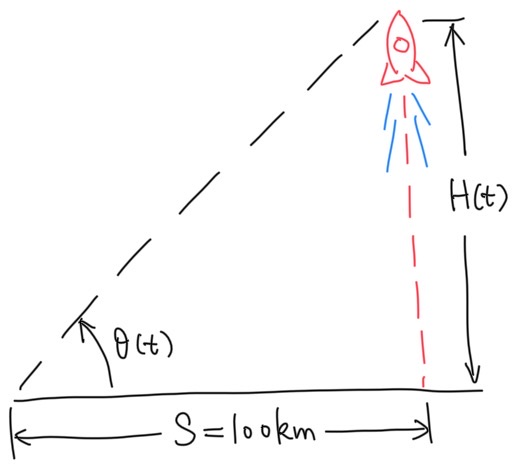
\includegraphics[width=5cm]{./images/ch2/Rocket.jpg}
		\column{0.6\textwidth}
		\pause 火箭的高度$H(t)=S\tan\theta(t)$,由此可知
		$$H'(t)=S\sec^2\theta(t)\theta'(t),$$
		\pause 将$S=100$,$\theta(t)=\df{\pi}4$,$\theta'(t)=0.1$代入即得
		指定时刻火箭上升的速率为$20$km/s。\hfill$\Box$
	\end{columns}
\end{frame}

\begin{frame}
	\linespread{1.5}
	\ba{3.长度为$6$米的梯子靠在墙角,梯子底部距离墙角$5$米,某一时刻梯子底部开始
	向远离墙角的方向滑动,滑动的速度为$0.2$米每秒,问
	\begin{enumerate}[(1)]
	  \setlength{\itemindent}{1cm}
	  \item 此时梯子顶部下滑的速度是多少?
	  \item 由梯子、墙面和地面构成的三角形的面积随时间的变化率是多少?
	  \item 梯子和地面的夹角的以怎样的速率变化?
	\end{enumerate}}	
\end{frame}

\begin{frame}
	\linespread{1.5}
	\small 解:\it
	如图,
	\begin{columns}
		\column{0.4\textwidth}
		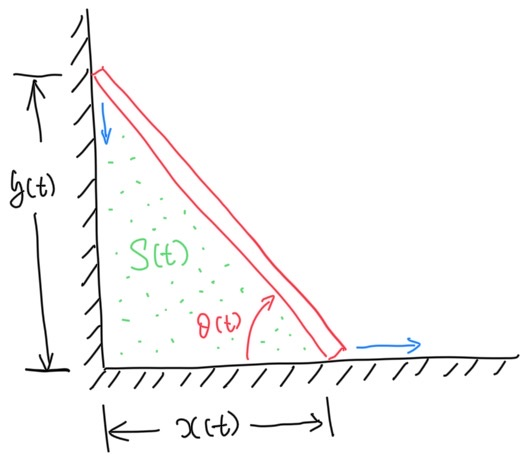
\includegraphics[width=5cm]{./images/ch2/ladder.jpg}
		\column{0.6\textwidth}
		\pause (1)显然$x^2(t)+y^2(t)=36$,两边求导可得
		$x'(t)x(t)+y'(t)y(t)=0$,进而
		$$y'(t)=-\df{x'(t)x(t)}{y(t)},$$
		\pause 代入$x(t)=5,x'(t)=0.2,y(t)=\sqrt{11}$,可得指定时刻
		梯子顶部的下滑速度为$-\df1{\sqrt{11}}$m/s;
	\end{columns}
\end{frame}

\begin{frame}
	\linespread{1.5}
	\small 解:\it
	如图,
	\begin{columns}
		\column{0.4\textwidth}
		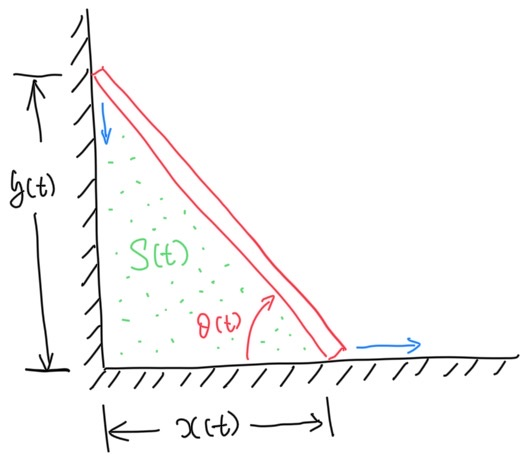
\includegraphics[width=5cm]{./images/ch2/ladder.jpg}
		\column{0.6\textwidth}
		(2)$S(t)=\df12x(t)y(t)$,故
		$$S'(t)=\df12[x'(t)y(t)+x(t)y'(t)],$$
		\pause 代入$x(t)=5,x'(t)=0.2,y(t)=\sqrt{11},y'(t)=-\df1{\sqrt{11}}$,
		可得所求三角形面积的变化速率为$-\df{7}{5\sqrt{11}}$m$^2$/s;
	\end{columns}
\end{frame}

\begin{frame}
	\linespread{1.5}
	\small 解:\it
	如图,
	\begin{columns}
		\column{0.4\textwidth}
		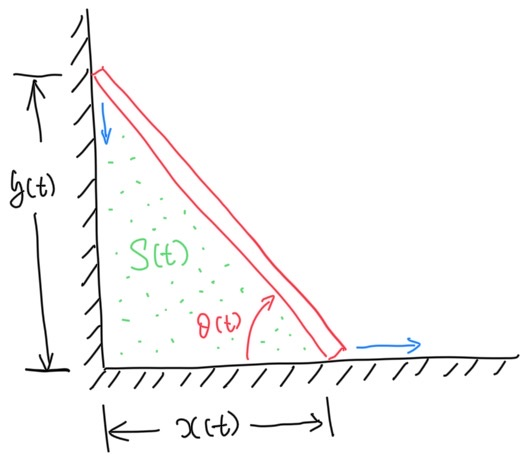
\includegraphics[width=5cm]{./images/ch2/ladder.jpg}
		\column{0.6\textwidth}
		(3)$\theta(t)=\arctan\df{y(t)}{x(t)}$,故
		$$\theta'(t)=\df1{1+\frac{y^2(t)}{x^2(t)}}
		=\df{y'(t)x(t)-y(t)x'(t)}{x^2(t)+y^2(t)},$$
		\pause 代入$x(t)=5,x'(t)=0.2,y(t)=\sqrt{11},y'(t)=-\df1{\sqrt{11}}$,
		可得指定时刻梯子和地面夹角的变化率为$-\df1{5\sqrt{11}}$弧度/s。\hfill$\Box$
	\end{columns}
\end{frame}

\begin{frame}
	\linespread{1.5}
	\ba{4.半径为$a$的圆球渐渐沉入盛有水的半径为$b(b>a)$的圆柱形容器中,若
	球的下降速度恒为$c$,求球浸没入水中恰好一半时,容器内水面上升的速率。
	}\pause
	
	\small 解:\it
	设$t$时刻,水中的球冠高度为$h(t)$,则此时水中的球冠体积
	$$V(t)=\df{\pi}3(3a-h(t))h^2(t),$$
	\pause 从而没入水中的球冠体积变换率
	$$V'(t)=\pi(2ah(t)-h^2(t))h'(t),$$
	\pause 相应地,桶内水面升高的速率为
	$$H'(t)=\df{V'(t)}{\pi [b^2-a^2+(a-h)^2]}
	=\df{2ah(t)-h^2(t)}{\pi [b^2-a^2+(a-h)^2]}h'(t),$$
	\pause 代入$h(t)=a,h'(t)=c$,即得所求水面上升的速率为$\df{a^2c}{b^2-a^2}$。
	\hfill$\Box$
\end{frame}